\chapter{Telematik}

Zusammenfassung der Vorlesung "`Telematik"' aus dem Wintersemester 2016.\footnote{\url{https://telematics.tm.kit.edu/ws201617_telematik.php}}

\section{Transportprotokolle}

\subsection{GrundlegendeKomponenten}

\subsubsection{TCP-Grundlagen}
\begin{itemize}
	\item \textbf{TCP-Verbindungsverwaltung}
	\begin{itemize}
		\item Identifikation einer TCP-Verbindung: Quell-/Zieladresse sowie Quell-/Zielport
		\item Verbindungsaufbau: Server wartet, Client initiiert Verbindung
		\item 3-Wege-Handshake
		\begin{enumerate}
			\item Client \(\rightarrow\) Server: \texttt{TConReq(SYN=1,seq=client\_isn)}
			\item Client \(\leftarrow\) Server: \texttt{TConCnf(SYN=1,ACK=1,seq=server\_isn,ack=client\_isn+1)}
			\item Client \(\rightarrow\) Server: \texttt{ACK(SYN=0,ACK=1,seq=client\_isn+1,ack=server\_isn+1)}
		\end{enumerate}
		\item Zusätzlich: Festlegen der initialen Sequenznummer (\texttt{isn}), Bekanntgabe der Größe des Flusskontrollfensters, Allokation der Puffer
		\item Format einer TCP-Dateneinheit\footnote{\url{https://upload.wikimedia.org/wikipedia/de/f/fd/TCP_Header.svg}}\\
			\begin{minipage}{\linewidth}
				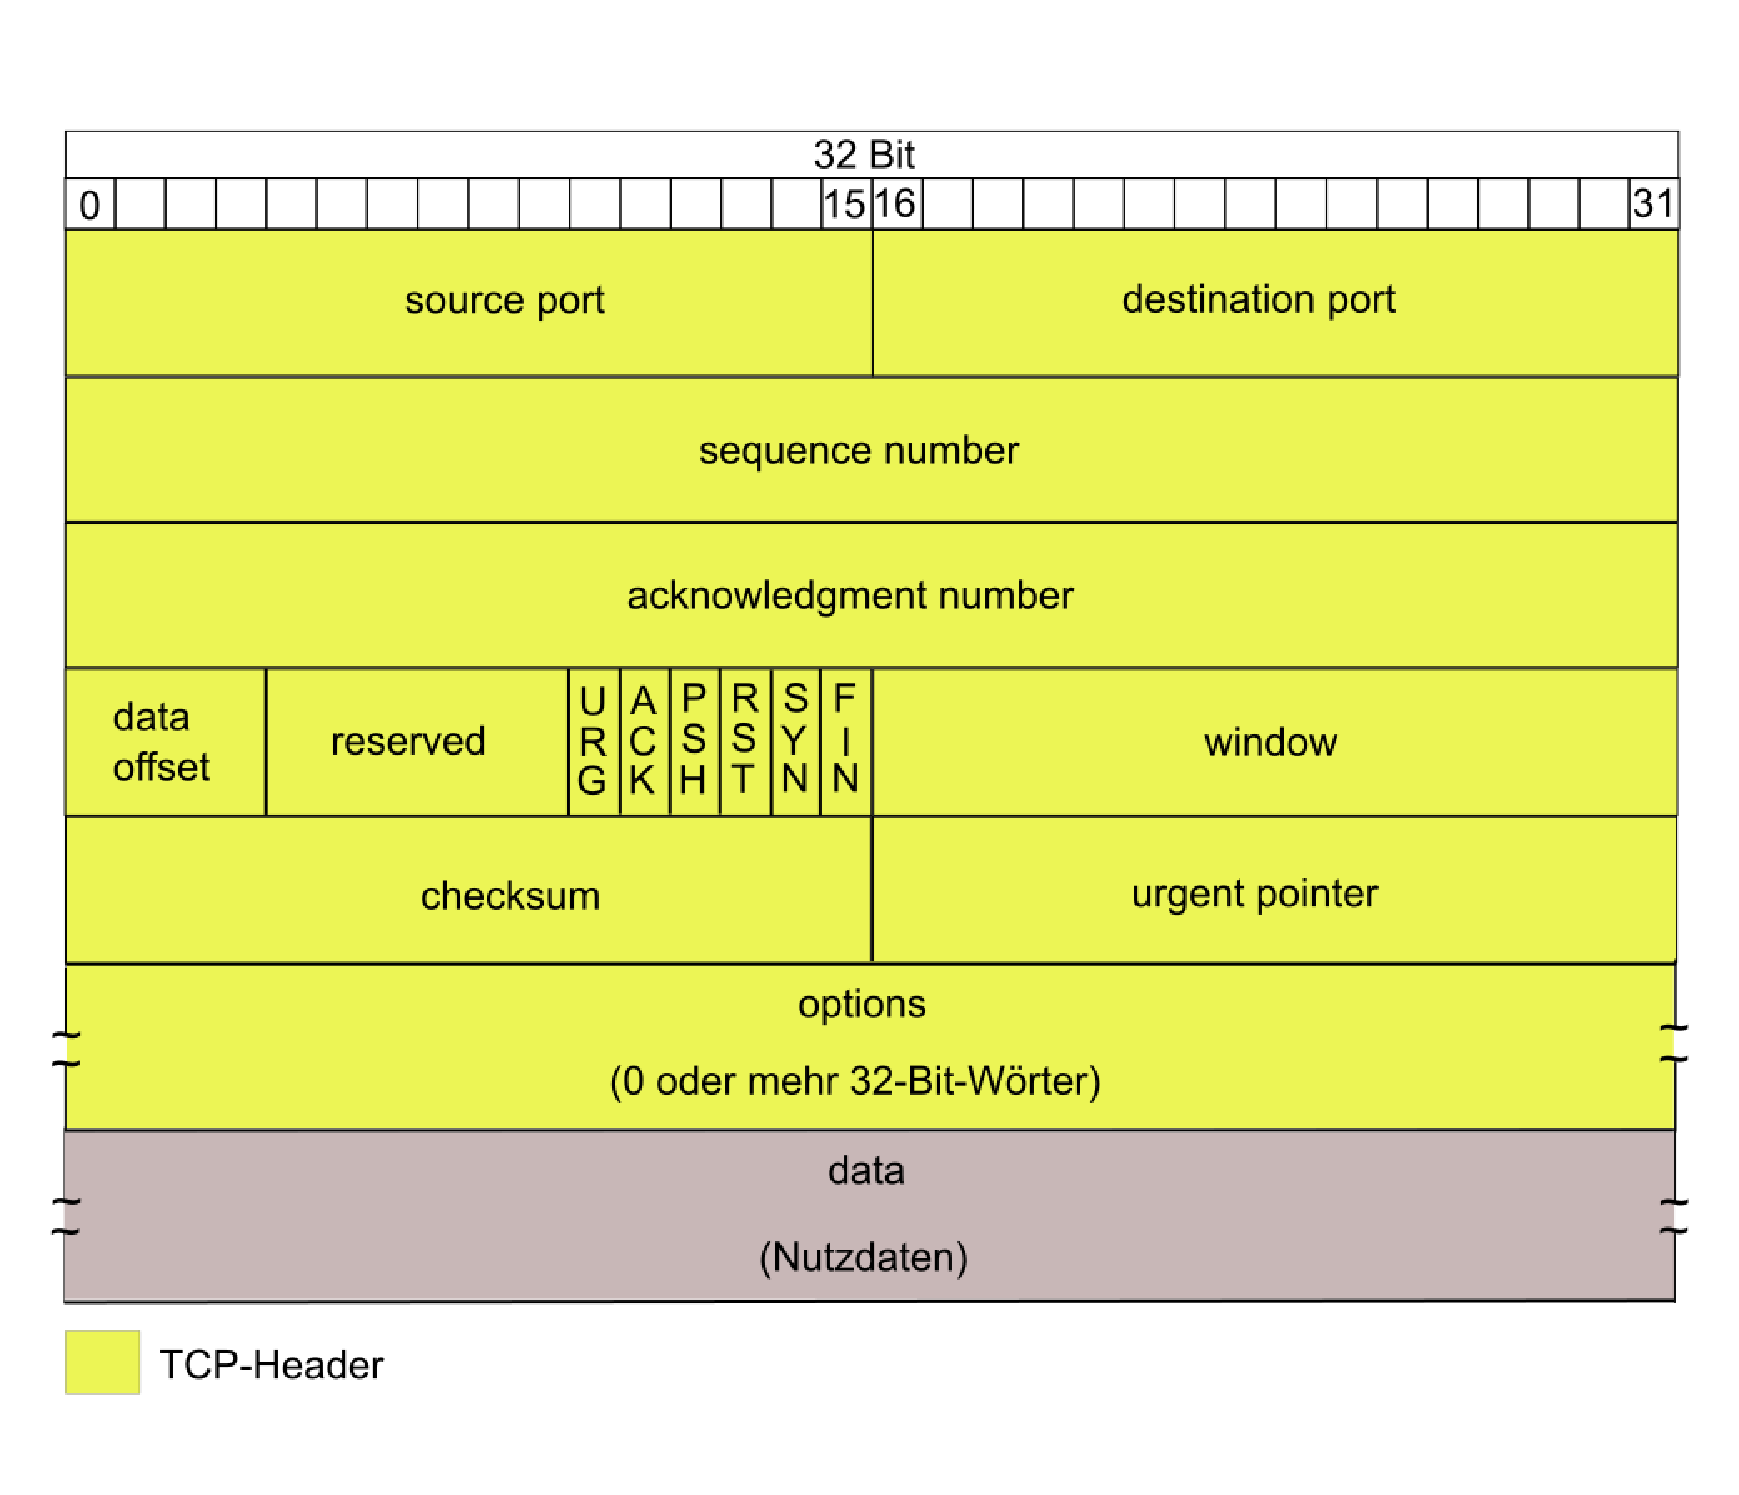
\includegraphics[scale=0.38]{telematik/TCP_Header.pdf}
			\end{minipage}
	\end{itemize}
	\item \textbf{Flusskontrolle zur Schutz des Empfängers vor zu hoher Last}
	\begin{itemize}
		\item Dynamische Anpassung des Empfangsfenster auf Empfängerseite, um die aktuelle verfügbare Puffergröße mitzuteilen. \texttt{RcvWindow} bezeichnet den Anteil des \texttt{RecvBuffer}, das frei ist (jeweils absolute Werte)
		\item Problem: \textit{Zero Window Probing}. Empfänger meldet ein volles Empfangsfenster. Wie weis der Sender, ab wann er wieder senden darf? Empfänger muss daher auch bei vollem Empfangsfenster Dateneinheiten mit einem Byte Länge quittieren
	\end{itemize}
	\item \textbf{Angriffe auf den Verbindungsaufbau: SYN-Flooding}
	\begin{itemize}
		\item Massenhaftes Senden von SYN-Dateneinheiten ohne Verbindungsaufbau. Problem: Zustandshaltung auf Empfängerseite für halboffene Verbindungen. Folge: Ressourcen erschöpft, Empfänger kann keine Dateneinheiten mehr annehmen
		\item Lösung: SYN-Cookies
		\begin{itemize}
			\item Verhinderung der Zustandshaltung bis zum letztmöglichen Zeitpunkt: Beginn der Zustandhaltung erst bei Empfang des \texttt{ACK}
			\item Realisierung: Ermittlung der Zustandsinformationen auf Empfängerseite anhand der Informationen aus \texttt{ACK(SYN=0,ACK=1,seq=client\_isn+1,ack=server\_isn+1)}
			\item Kodierungsbeispiel: Zeitstempel zur Verhinderung von Replay-Attacken (5 Bit); ausgewählte MSS aus acht vordefinierten Werten (3 Bit); Hash über Quelladresse und -port sowie Zieladresse und -port, verifiziert dass der Client bereits \texttt{SYN} durchgeführt hat /24 Bit). Daraus entsteht die 32 Bit initiale Sequenznummer des Servers
			\item Nachteil: Vergleichsweise kurze Sequenznummer reicht nicht für zusätzliche TCP-Optionen und limitiert MSS-Größen auf vordefinierte Werte
			\item Idee: Cookie erst einsetzen, wenn nötig (volle Warteschlange oder Ressourcenengpass)
		\end{itemize}
	\end{itemize}
\end{itemize}

\subsubsection{Staukontrolle}
\begin{itemize}
	\item Beobachtung: Unverhältnismäßiger Leistungseinbruch an Engstellen bei großem Datenaufkommen zwischen zwei schnelleren Netzen \(\rightarrow\) Warteschlangenmanagement notwendig
	\item \textbf{Einfaches Warteschlangenmanagement}
	\begin{itemize}
		\item Puffer im Router voll, nächste Dateneinheit muss verworfen werden ("`Tail Drop"'
		')
		\item Retransmissiontimer im Client steuert Sendewiederholungen
		\item Problem: Synchronisation. Dateineinheiten von mehreren Verbindungen werden quasi gleichzeitig verworfen
	\end{itemize}
	\item \textbf{Aktives Warteschlangenmanagement}
	\begin{itemize}
		\item Das Netz gibt einen Hinweis auf eine entstehende Stausituation
		\item Router verwirft (randomisiert) Dateneinheiten, bevor die Warteschlange voll ist
		\item Verfahren
		\begin{itemize}
			\item Konkrete Implementierung: Random Early Detection (RED)
			\begin{itemize}
				\item Wahrscheinlichkeit, dass eine Dateneinheit verworfen wird, steigt linear mit der Warteschlangenlänge
			\end{itemize}
		\end{itemize}
	\end{itemize}
	\item \textbf{Self-Clocking}
	\begin{itemize}
		\item Szenario: Verbindung zweier Netze über langsames Weitverkehrsnetz. Dateneinheiten benötigen bei der langsamen Übertragung mehr Zeit als in den lokalen Netzen. Dadurch kommen sie verzögert beim Empfänger an, welcher sie entsprechend "`langsam"' quittiert. Durch den entstehenden Takt weis der Sender, wie schnell er senden kann. Aber: Wie soll die "`Uhr"' gestartet werden
		\item Wieso wird kein Gleichgewicht erreicht?
		\begin{itemize}
			\item Verbindung kommt nicht ins Gleichgewicht. Mögliche Auslöser: Neue Verbindung/Neustart, automatische Anpassung der Datenrate und Verzögerung
			\item Sender sendet neue Dateneinheiten zu früh
			\item Ressourcenbeschränkungen verhindern Gleichgewicht
		\end{itemize}
		\item Slow-Start (Einzelverbindung)
		\begin{itemize}
			\item Erhöhung der Anzahl der gesendeten Dateneinheiten über die Zeit durch Einführung eines Staukontrollfensters (\texttt{Staukontrollfenster < Flusskontrollfenster}). Verhindert burstartiges Senden der Quelle, was zu vielen Sendewiederholungen führen würde
			\item Startverhalten ohne Slow-Start: Viele Sendewiederholungen durch Paketverluste. "`lineares Zickzackwachstum"', das weit hinter der verfügbaren Datenrate zurück bleibt (effektive Nutzung bei 35\%)
			\item Startverhalten mit 2s Slow-Start: Keine Sendewiederholungen, Datenrate nahezu am verfügbaren Maximum. Effiziens abhängig von Vebrindungsdauer, da dann die langsame Slow-Start-Phase an Gewicht verliert
		\end{itemize}
		\item Congestion Avoidence (Simultane, konkurrierende Verbindungen)
		\begin{itemize}
			\item Ohne Congestion Avoidance: Sehr viele Sendewiederholungen (nahezu 50\% im Experiment), sehr unfaire Aufteilung
			\item Mit Congestion Avoidance: Sehr wenige Sendewiederholungen, verschiedene Quittungsstrategien möglich
			\item Zusammenfassung: Faire Aufteilung der verfügbaren Kapazität, langsames Herantasten durch lineares Erhöhen des Staukontrollfensters sowie kaum Sendewiederholungen
		\end{itemize}
		\item Fast Retransmit
		\begin{itemize}
			\item Beobachtung: Nicht jede nicht in Reihenfolge erhaltene Dateneinheit ist ein Indiz für eine Überlastung des Netzes
			\item Mechanismus zur Staukontrolle: Sendewiederholung beim Empfangeiner defiierten Anzahl duplizierter Quittungen
			\item Vorgehen: Warten auf Timerablauf, dann Sendewiederholung (Wartezeit größer Umlaufzeit \texttt{RTT})
		\end{itemize}
	\end{itemize}
	\item \textbf{Staukontrolle}
	\begin{itemize}
		\item Implizite Staukontrolle: Implizite "`Anzeige"' einer Stausituation ohne explizite Unterstützung des Netzes
		\begin{enumerate}
			\item TCP-Tahoe
			\begin{itemize}
				\item Mechanismen: Slow Start, Timeout, Congestion Avoidance, Fast Retransmit
				\item Nach Timeout oder Empfang duplizirter Quittungen: Beginn von Slow Start
				\item Grundlegende Vorgehensweise: Additives Erhöhen des Congestion Window \texttt{CWnd}, multiplikatives Erniedrigen (\texttt{AIMD})
			\end{itemize}
			\item TCP-Reno
			\begin{itemize}
				\item Zusätzlich zu TCP-Tahoe: Fast Recovery (siehe unten)
				\item Unterscheidet zwischen \textit{schweren Stausituationen} (Timeout bei Ausstehenden Quittungen) und \textit{leichten Stausituationen} (Empfang von duplizierten Quittungen)
				\item Leichte Stausituationen: Kein Rücksetzen auf Slow Start, da Quittungsempfang impliziert, dass weiter neue Daten empfangen worden sind
				\item Schwere Stausituationen: Rücksetzen auf Slow Start wie bei TCP-Tahoe
				\item Fast Recovery
				\begin{itemize}
					\item Szenario: Empfang einer festgelegten Anzahl Quittungen (beispielsweise drei)
					\item Idee: Senden neuer Dateneinheiten, auch wenn der Fehler noch nicht behoben ist (Self-Clocking geht weiter)
					\item Vorgehen: Reduzierung der Belastung (halbieren des Staukontrollfensters) sowie Fast Retransmit
				\end{itemize}
			\end{itemize}
		\end{enumerate}
		\item Explizit Congestion Notification (ECN): Explizite Staukontrolle mit Netzunterstützung
		\begin{itemize}
			\item Idee: Erkennen von Stausituationen im Netz über den Füllstand der Warteschlange (setzt aktives Warteschlangenmanagement voraus) sowie markieren der IP-Einheiten vor Weiterleitung zum Empfänger. Dieser informiert den Sender, um das Staukontrollfenster zu regeln
			\item Signalisierung in Schicht 3 (IP): Nutzung zweier Bits im TOS-Feld der Dateneinheit
			\item Signailisierung in Schicht 4 (TCP): Einführung zusätzlicher Flags im TCP-Kopf
			\begin{itemize}
				\item \texttt{ECE}-Bit: Signalisiert dem Sender die Stausituation (Sender \(\leftarrow)\) Empfänger)
				\item \texttt{CWR}-Bit: Bestätigt dem Empfänger den Erhalt einer Staumeldung (Sender \(rightarrow\) Empfänger)
			\end{itemize}
		\end{itemize}
	\end{itemize}
\end{itemize}

\subsubsection{Fairness}
\begin{itemize}
	\item TCP-Verbindungen konkurrieren um Ressourcen des Netzes \(rightarrow\) faire Aufteilung angestrebt
	\item \textbf{Probleme}
	\begin{itemize}
		\item "`Gierige Nutzer"': Faire Verteilung bezieht sich auf TCP-Verbindungen. Kann daher mehrere Verbindungen gleichzeitig öffnen. Gegenmaßnahme: Verteilung der Kapazität pro Benutzer
		\item "`Gieriger Empfänger"': Da Quittungsverhalten der Empfängerinstanz die Ressourcenzuteilung beeinflusst, kann dieser mehr oder scheller Quittungen senden. Das Staukontrollfenster öffnet sich schneller, damit erhält die Verbindung mehr Ressourcen
		\begin{enumerate}
			\item Mehrere Quittungen pro empfangener Dateneinheit: Sequenznummern zählen Bytes, Staukontrollfenster zählen Dateneinheiten. Bestätigt der Empfänger jede Dateneinheit in mehreren "`Häppchen"', so öffnet sich das Staukontrollfenster schneller
			\item Quittungen schneller senden als Daten empfangen werden. Protokolländerung notwendig
			\item Identische Quittungen mehrfach senden: Fehlende Dateneinheit wird erneut gesendet. Bei TCP-Reno läuft Self-Clocking weiter \(\rightarrow\) Staukontrollfenster wird weiter geöffnet
		\end{enumerate}
	\end{itemize}
\end{itemize}

\subsection{Analyse und Randbedingungen}


\subsection{Aktuelle Entwicklungen}
